% Options for packages loaded elsewhere
\PassOptionsToPackage{unicode}{hyperref}
\PassOptionsToPackage{hyphens}{url}
\PassOptionsToPackage{dvipsnames,svgnames,x11names}{xcolor}
%
\documentclass[
  letterpaper,
  DIV=11,
  numbers=noendperiod]{scrreprt}

\usepackage{amsmath,amssymb}
\usepackage{iftex}
\ifPDFTeX
  \usepackage[T1]{fontenc}
  \usepackage[utf8]{inputenc}
  \usepackage{textcomp} % provide euro and other symbols
\else % if luatex or xetex
  \usepackage{unicode-math}
  \defaultfontfeatures{Scale=MatchLowercase}
  \defaultfontfeatures[\rmfamily]{Ligatures=TeX,Scale=1}
\fi
\usepackage{lmodern}
\ifPDFTeX\else  
    % xetex/luatex font selection
\fi
% Use upquote if available, for straight quotes in verbatim environments
\IfFileExists{upquote.sty}{\usepackage{upquote}}{}
\IfFileExists{microtype.sty}{% use microtype if available
  \usepackage[]{microtype}
  \UseMicrotypeSet[protrusion]{basicmath} % disable protrusion for tt fonts
}{}
\makeatletter
\@ifundefined{KOMAClassName}{% if non-KOMA class
  \IfFileExists{parskip.sty}{%
    \usepackage{parskip}
  }{% else
    \setlength{\parindent}{0pt}
    \setlength{\parskip}{6pt plus 2pt minus 1pt}}
}{% if KOMA class
  \KOMAoptions{parskip=half}}
\makeatother
\usepackage{xcolor}
\setlength{\emergencystretch}{3em} % prevent overfull lines
\setcounter{secnumdepth}{5}
% Make \paragraph and \subparagraph free-standing
\ifx\paragraph\undefined\else
  \let\oldparagraph\paragraph
  \renewcommand{\paragraph}[1]{\oldparagraph{#1}\mbox{}}
\fi
\ifx\subparagraph\undefined\else
  \let\oldsubparagraph\subparagraph
  \renewcommand{\subparagraph}[1]{\oldsubparagraph{#1}\mbox{}}
\fi


\providecommand{\tightlist}{%
  \setlength{\itemsep}{0pt}\setlength{\parskip}{0pt}}\usepackage{longtable,booktabs,array}
\usepackage{calc} % for calculating minipage widths
% Correct order of tables after \paragraph or \subparagraph
\usepackage{etoolbox}
\makeatletter
\patchcmd\longtable{\par}{\if@noskipsec\mbox{}\fi\par}{}{}
\makeatother
% Allow footnotes in longtable head/foot
\IfFileExists{footnotehyper.sty}{\usepackage{footnotehyper}}{\usepackage{footnote}}
\makesavenoteenv{longtable}
\usepackage{graphicx}
\makeatletter
\def\maxwidth{\ifdim\Gin@nat@width>\linewidth\linewidth\else\Gin@nat@width\fi}
\def\maxheight{\ifdim\Gin@nat@height>\textheight\textheight\else\Gin@nat@height\fi}
\makeatother
% Scale images if necessary, so that they will not overflow the page
% margins by default, and it is still possible to overwrite the defaults
% using explicit options in \includegraphics[width, height, ...]{}
\setkeys{Gin}{width=\maxwidth,height=\maxheight,keepaspectratio}
% Set default figure placement to htbp
\makeatletter
\def\fps@figure{htbp}
\makeatother
\newlength{\cslhangindent}
\setlength{\cslhangindent}{1.5em}
\newlength{\csllabelwidth}
\setlength{\csllabelwidth}{3em}
\newlength{\cslentryspacingunit} % times entry-spacing
\setlength{\cslentryspacingunit}{\parskip}
\newenvironment{CSLReferences}[2] % #1 hanging-ident, #2 entry spacing
 {% don't indent paragraphs
  \setlength{\parindent}{0pt}
  % turn on hanging indent if param 1 is 1
  \ifodd #1
  \let\oldpar\par
  \def\par{\hangindent=\cslhangindent\oldpar}
  \fi
  % set entry spacing
  \setlength{\parskip}{#2\cslentryspacingunit}
 }%
 {}
\usepackage{calc}
\newcommand{\CSLBlock}[1]{#1\hfill\break}
\newcommand{\CSLLeftMargin}[1]{\parbox[t]{\csllabelwidth}{#1}}
\newcommand{\CSLRightInline}[1]{\parbox[t]{\linewidth - \csllabelwidth}{#1}\break}
\newcommand{\CSLIndent}[1]{\hspace{\cslhangindent}#1}

\KOMAoption{captions}{tableheading}
\makeatletter
\makeatother
\makeatletter
\@ifpackageloaded{bookmark}{}{\usepackage{bookmark}}
\makeatother
\makeatletter
\@ifpackageloaded{caption}{}{\usepackage{caption}}
\AtBeginDocument{%
\ifdefined\contentsname
  \renewcommand*\contentsname{Table of contents}
\else
  \newcommand\contentsname{Table of contents}
\fi
\ifdefined\listfigurename
  \renewcommand*\listfigurename{List of Figures}
\else
  \newcommand\listfigurename{List of Figures}
\fi
\ifdefined\listtablename
  \renewcommand*\listtablename{List of Tables}
\else
  \newcommand\listtablename{List of Tables}
\fi
\ifdefined\figurename
  \renewcommand*\figurename{Figure}
\else
  \newcommand\figurename{Figure}
\fi
\ifdefined\tablename
  \renewcommand*\tablename{Table}
\else
  \newcommand\tablename{Table}
\fi
}
\@ifpackageloaded{float}{}{\usepackage{float}}
\floatstyle{ruled}
\@ifundefined{c@chapter}{\newfloat{codelisting}{h}{lop}}{\newfloat{codelisting}{h}{lop}[chapter]}
\floatname{codelisting}{Listing}
\newcommand*\listoflistings{\listof{codelisting}{List of Listings}}
\makeatother
\makeatletter
\@ifpackageloaded{caption}{}{\usepackage{caption}}
\@ifpackageloaded{subcaption}{}{\usepackage{subcaption}}
\makeatother
\makeatletter
\@ifpackageloaded{tcolorbox}{}{\usepackage[skins,breakable]{tcolorbox}}
\makeatother
\makeatletter
\@ifundefined{shadecolor}{\definecolor{shadecolor}{rgb}{.97, .97, .97}}
\makeatother
\makeatletter
\makeatother
\makeatletter
\makeatother
\ifLuaTeX
  \usepackage{selnolig}  % disable illegal ligatures
\fi
\IfFileExists{bookmark.sty}{\usepackage{bookmark}}{\usepackage{hyperref}}
\IfFileExists{xurl.sty}{\usepackage{xurl}}{} % add URL line breaks if available
\urlstyle{same} % disable monospaced font for URLs
\hypersetup{
  pdftitle={Computational Methods for human population genetics and ancient DNA},
  pdfauthor={Various enthusiasts at the MPI-EVA},
  colorlinks=true,
  linkcolor={blue},
  filecolor={Maroon},
  citecolor={Blue},
  urlcolor={Blue},
  pdfcreator={LaTeX via pandoc}}

\title{Computational Methods for human population genetics and ancient
DNA}
\author{Various enthusiasts at the MPI-EVA}
\date{2023-09-21}

\begin{document}
\maketitle
\ifdefined\Shaded\renewenvironment{Shaded}{\begin{tcolorbox}[boxrule=0pt, sharp corners, breakable, borderline west={3pt}{0pt}{shadecolor}, frame hidden, enhanced, interior hidden]}{\end{tcolorbox}}\fi

\renewcommand*\contentsname{Table of contents}
{
\hypersetup{linkcolor=}
\setcounter{tocdepth}{2}
\tableofcontents
}
\bookmarksetup{startatroot}

\hypertarget{preface}{%
\chapter*{Preface}\label{preface}}
\addcontentsline{toc}{chapter}{Preface}

\markboth{Preface}{Preface}

This book summarises prepared mini-courses for various computational
tools and methods in the field of human archaeogenetic data analysis,
with a particular emphasis on population genetics.

The chapters are contributed by different authors, as indicated in the
Yaml-frontmatter of each chapter's \texttt{.qmd} source file.

\bookmarksetup{startatroot}

\hypertarget{introduction-to-quarto}{%
\chapter{Introduction to Quarto}\label{introduction-to-quarto}}

In this introduction to quarto, you will be shown the basics in how to
set up a website and a book. For more detailed information, I highly
recommend checking out the \href{https://quarto.org}{website} and also
watch the \href{https://youtu.be/_f3latmOhew}{introduction tutorial}.

\hypertarget{setting-up}{%
\section{Setting up}\label{setting-up}}

Quarto is the ``next generation'' of R Markdown and is usable on
different tools.

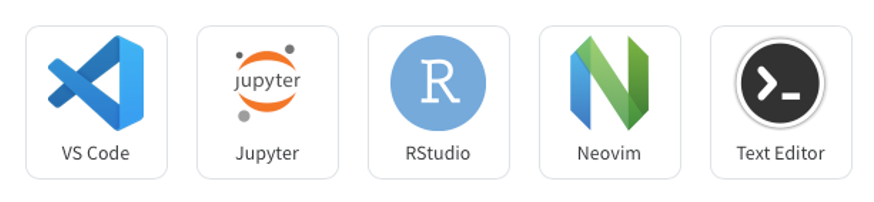
\includegraphics[width=3.125in,height=\textheight]{img/quarto_intro/Picture 1.png}

Here, we will describe how to set up your environment to use Quarto in
\textbf{RStudio}, and VSCode.

Quarto in general is set up to be very intuitive and user friendly. And
while it is possible to set up different documents simultaneously, those
can also easily be set up to in just the way you need for whatever
occasion. So, for either communicating your results to collaborators,
discuss code with your supervisor, setting up a website or writing your
paper, to just name some scenarios, quarto comes in quite handy. So,
let's begin:

\hypertarget{rstudio}{%
\section{RStudio}\label{rstudio}}

For this, you have to
\href{https://posit.co/download/rstudio-desktop/}{download} RStudio
first. If you have done this already, we can get started.

\hypertarget{getting-started}{%
\subsection{Getting started}\label{getting-started}}

First, we have to install the quarto package using the following command
in our console:

\texttt{install.packages("quarto")}

Now we are ready to set up a quarto document.

For this we open a new project and select the quarto document we want to
create. You can choose to set up a git repository as well. For
practicality, I usually also tick the box visual markdown editor.

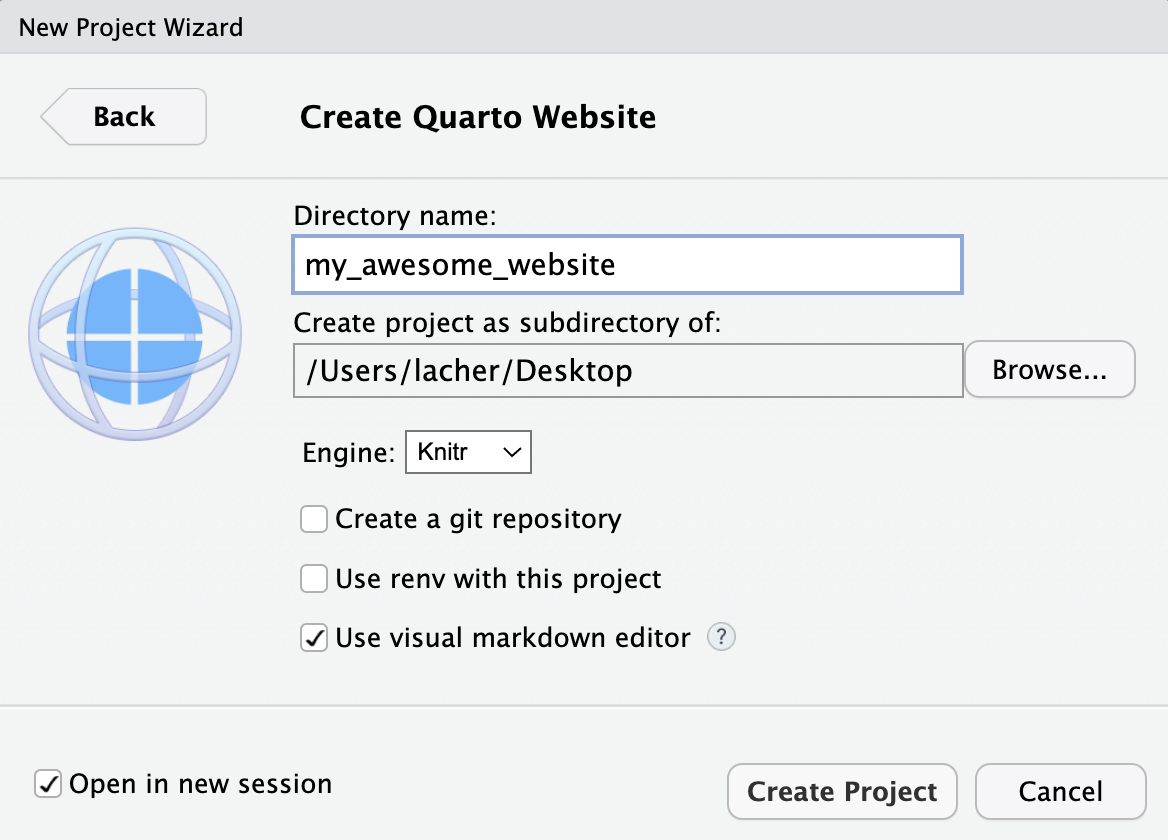
\includegraphics[width=3.125in,height=\textheight]{img/quarto_intro/Screenshot 2023-10-11 at 11.34.16.png}

The new project will look like this:

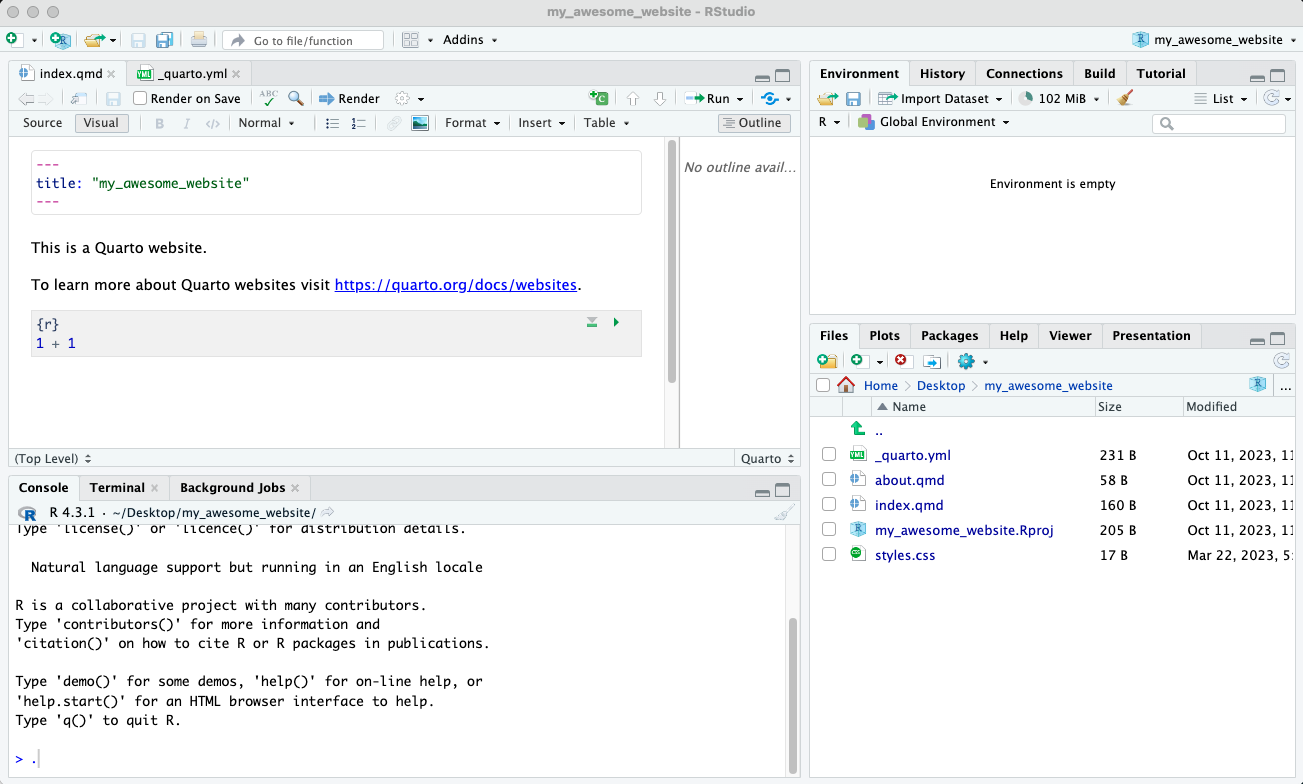
\includegraphics{img/quarto_intro/Screenshot 2023-10-11 at 11.39.43.png}

\hypertarget{universal-instructions}{%
\subsection{Universal instructions}\label{universal-instructions}}

When setting up your document, quarto will always provide you with some
presets. So first, we will have a look into the .qmd files, for they are
handled the same way, regardless the format you are setting up (website,
book, presentation, etc.).

\hypertarget{render-save}{%
\subsubsection{Render \& save}\label{render-save}}

If we now click on render, we will be provided with the preview of our
final version if the project in the viewer.

\textbf{Important: Do not mistake ``save'' with ``render''.} Just by
saving, your document did not get rendered automatically,
\textbf{unless} you tick the box ``\textbf{Render on Save}''. You have
to tick that box on each .qmd file individually though.

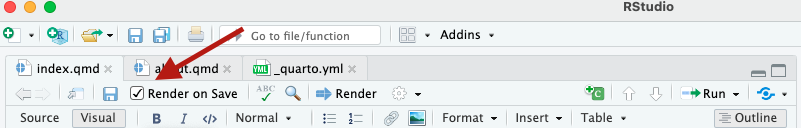
\includegraphics[width=3.125in,height=\textheight]{img/quarto_intro/Screenshot 2023-10-11 at 14.12.45.png}

\hypertarget{visual-and-source}{%
\subsubsection{Visual and Source}\label{visual-and-source}}

If you have chosen the \textbf{Visual} option on your toolbar, the
preview will mostly resemble your .qmd files. If you are more
comfortable with the R markdown optics, you can switch to
\textbf{Source.}

In the \textbf{Source} version, you can write up your document in LaTeX.

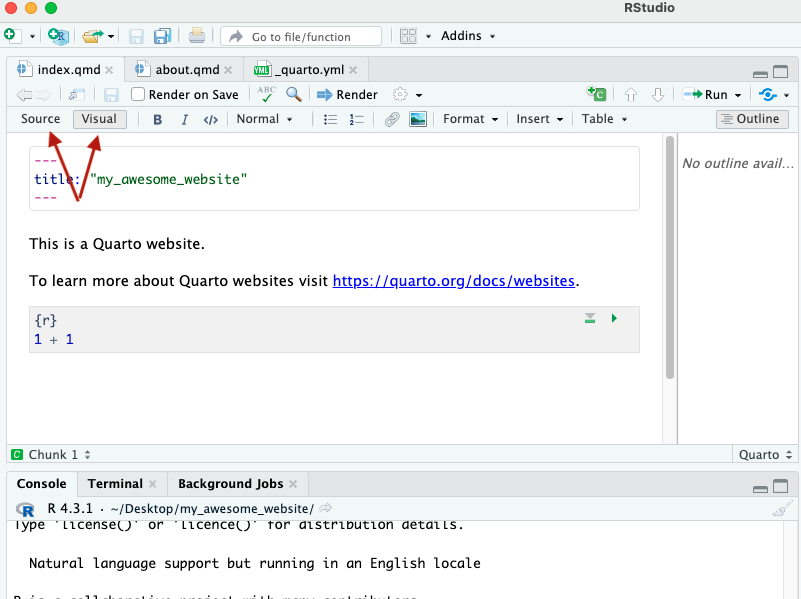
\includegraphics[width=4.16667in,height=\textheight]{img/quarto_intro/Screenshot_3.png}

\hypertarget{qmd-files}{%
\subsubsection{.qmd files}\label{qmd-files}}

Quarto will automatically provide you with two \textbf{.qmd files}, as
well as a \textbf{.yml file}.

The .qmd files respond to the individual pages of your website or
chapter of your book or pages of your presentation, etc. You can shape
them individually or define the layout for all of them in the .yml file,
to which we will get later.

In your .qmd files you also find a yaml at the top of your document,
separated by

-\/-\/-

-\/-\/-

Within these, you can define the outline of .qmd file
\textbf{individually}, starting with the page header. Other options, you
might be using in the future are:

\texttt{author:\ Jessi\ Doe}

-\textgreater{} will add an author underneath the header

\texttt{execute:\ \ \ \ echo:\ true}

-\textgreater{} if \textgreater true\textless, code will be visible

\texttt{toc:true}

-\textgreater{} if \textgreater true\textless, a table of content will
be automatically added

\texttt{bibliography:\ your\_references.bib}

-\textgreater{} file or list of files for your references

It is crucial to stick to the spacing. Otherwise, an error will occur.

\hypertarget{insert}{%
\paragraph{Insert}\label{insert}}

If you click \texttt{Insert}, you will realize, quarto provides you with
a lot of options and shortcuts as well. So by just selecting on your
chosen item to insert, it will be added to the document, while you are
also provided with options on the appearance (in the case of
figure/images or tables, etc). We will here have a brief look into how
to work with \textbf{R code} and how to use the \textbf{reference}
option.

\hypertarget{r-code}{%
\paragraph{R code}\label{r-code}}

To add R code to your file, you select \texttt{Insert}, select
\texttt{Code\ Cell} and choose the kind of code you want to insert. In
this case, \texttt{R}. There are some things to keep in mind though.

Depending on how you have set up your .qmd file (or your .yml), your
code will be visible or not on your website. To check your output, you
can click the green arrow for the latest bit of code or the grey arrow
above a bar to run the previous code.

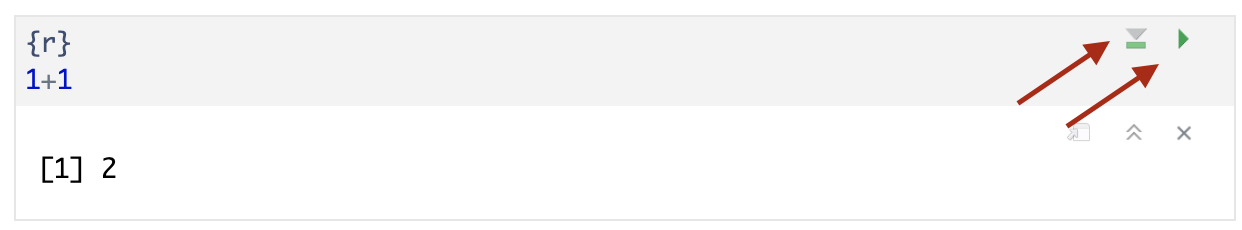
\includegraphics[width=4.16667in,height=\textheight]{img/quarto_intro/Screenshot 2023-10-11 at 15.04.31.png}

But in case there are some chunks of code, you do not want to show all
the time, there are some nice sets.

So if we just load the library \texttt{tidyverse}, for example, the
additional information regardless and it will be also visible on our
website.

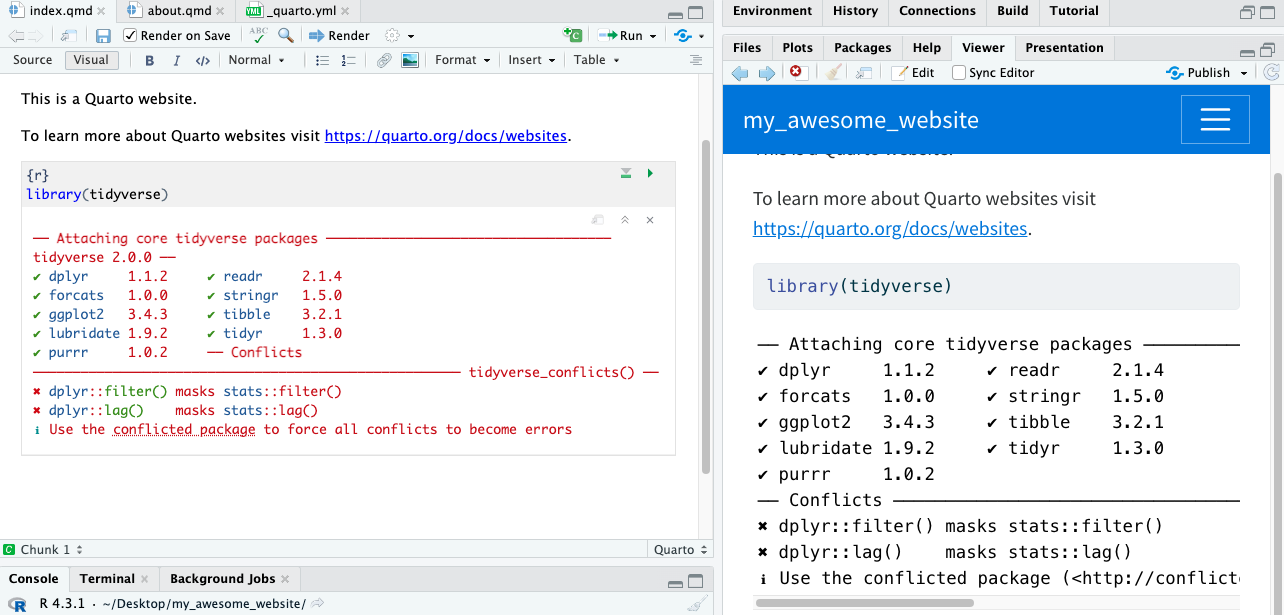
\includegraphics{img/quarto_intro/Screenshot 2023-10-11 at 14.49.43.png}

To avoid this, we can set up a code chunk, looking like this:

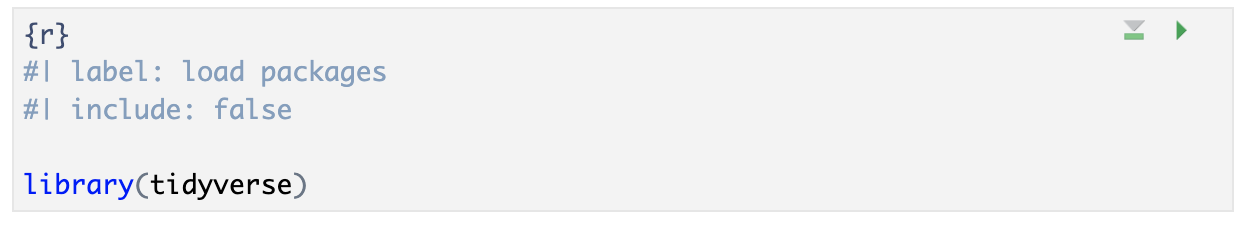
\includegraphics{img/quarto_intro/Screenshot 2023-10-11 at 14.55.13.png}

This will prevent the output of this code chunk to be depicted on your
website, while the package is otherwise active and can be used in the
following R code. This is, by the way, true for all R code and data sets
you will use: they will be active in your document and can be used in
different code chunks, once provided.

A code block included in your document could look like the following.
Here I used the option

\texttt{code-fold:\ true} so the code can be extended. This option is
only available in html though.

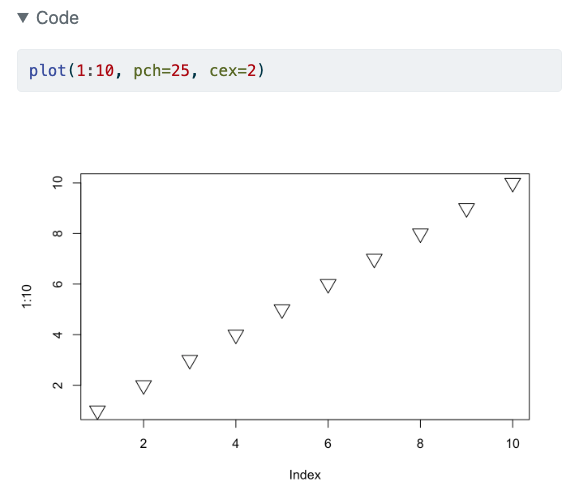
\includegraphics[width=4.16667in,height=\textheight]{img/quarto_intro/Screenshot 2023-10-17 at 17.05.28.png}

\hypertarget{references}{%
\paragraph{References}\label{references}}

Depending on which citation program you are using, quarto is able to
connect to it (\href{https://www.zotero.org}{Zotero} works, for
example). So, when selecting to insert a \texttt{Citation}, you can
choose to simply add a reference from your program.

Alternatively, you are provided with some options to choose from:

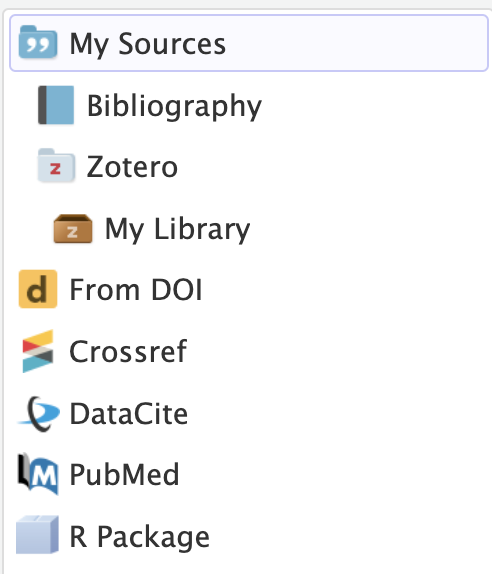
\includegraphics[width=2.08333in,height=\textheight]{img/quarto_intro/Screenshot 2023-10-11 at 15.09.41.png}

In your source code and your website, a citation will be depicted as
follows:


\includegraphics{img/quarto_intro/Screenshot 2023-10-11 at 15.12.57.png}

The citation will also automatically be added to a
\texttt{references.bib} as well as to a \texttt{references.qmd} and is
therefore available on your website on the page ``References'', which
also will be created automatically.

\hypertarget{render-your-document}{%
\subsection{Render your document}\label{render-your-document}}

When done with setting up your documents, you would like to have the
actual output. Depending on the \texttt{format} you set in your .yml
file, your output can be a \texttt{html}, \texttt{pdf},
\texttt{MS\ Word}, \texttt{OpenOffice}, or \texttt{ePUB} file. To create
those, the terminal in your RStudio Project is used.

By using the command:\\
\texttt{quarto\ render}

all formats you predefined in your .yml file will be rendered.

In case you are only interested in one format to be rendered, you can
specify your command:

\texttt{quarto\ render\ -to\ pdf}

Your rendered document should now look like this:

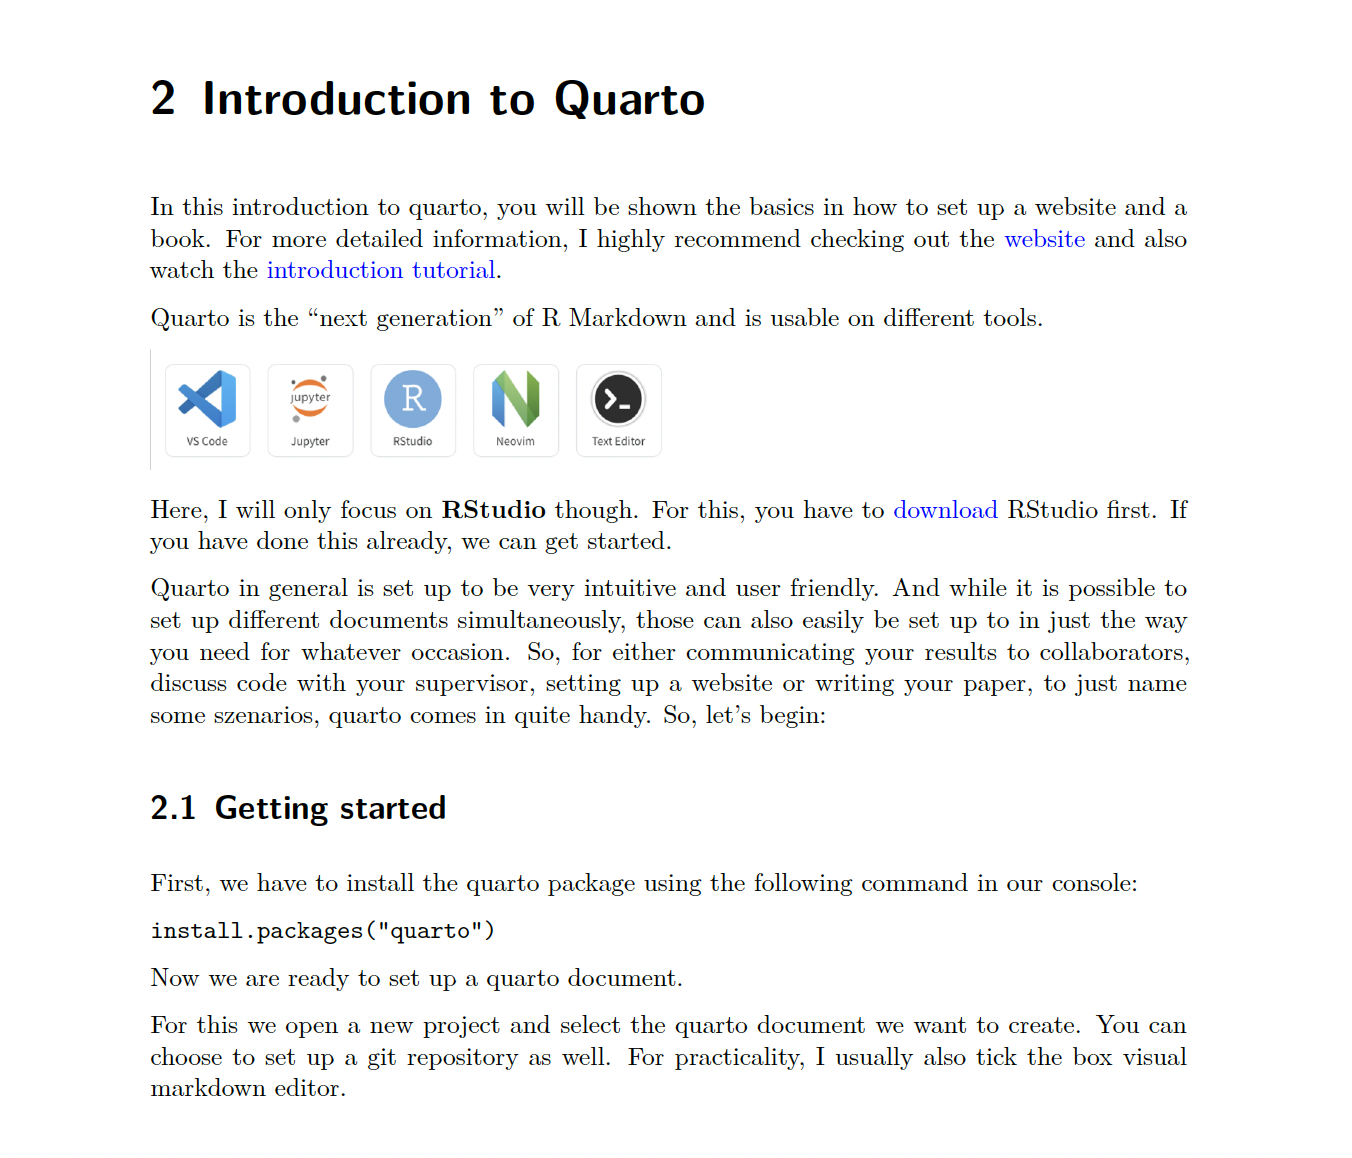
\includegraphics{img/quarto_intro/Screenshot 2023-10-17 at 14.15.05.png}

\hypertarget{quarto-website}{%
\subsection{Quarto website}\label{quarto-website}}

In the provided .qmd files, the index is also the first page of your
website. As you might have noticed, quarto already sets up a navbar as
well as a search function on your website.

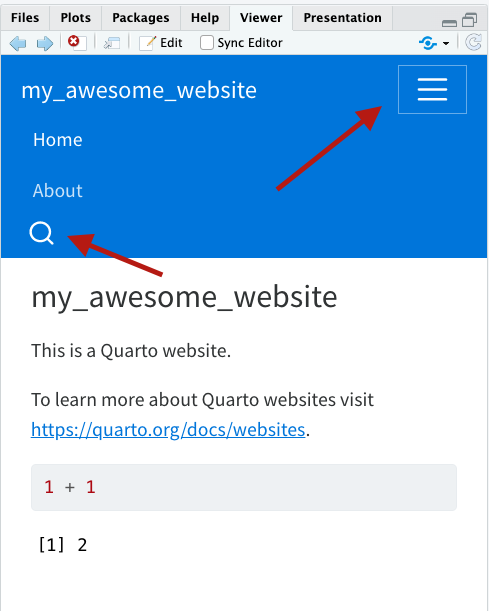
\includegraphics[width=2.08333in,height=\textheight]{img/quarto_intro/Screenshot 2023-10-11 at 14.09.08.png}

\hypertarget{yml-files}{%
\subsubsection{.yml files}\label{yml-files}}

While your .qmd files contain information about one page, the .yml file
defines the overall looks of the website.

Here, you can define the type of your project (in this case a website),
you can change the name of the website (\texttt{Title}), define your
navbar (which shall be your landing page and in what order your pages
shall be set up) or the overall appearance of your website in general
(\texttt{theme}, \texttt{css}, \texttt{toc}, \texttt{backgroundcolor},
etc.). For different styles and layouts, check out the quarto
\href{https://quarto.org/docs/reference/formats/html.html}{website}
again.

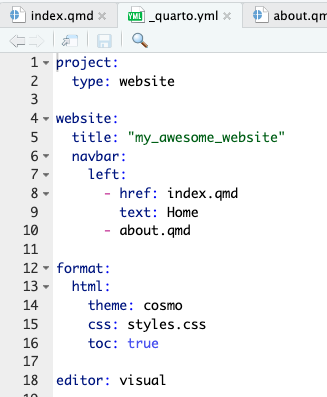
\includegraphics[width=2.08333in,height=\textheight]{img/quarto_intro/Screenshot 2023-10-12 at 11.25.37.png}

\hypertarget{quarto-book}{%
\subsection{Quarto book}\label{quarto-book}}

The setup of the .yml file in a quarto book is slightly different than
that of the website. So here are some general remarks about them.

\hypertarget{yml-files-1}{%
\subsubsection{.yml files}\label{yml-files-1}}

We see, for example, that instead of a navbar, we find
\texttt{chapters}. Those will appear in the listed order in your book.

We also already get provided with a \texttt{bibliography} and the
responding .bib file. If you have other .bib files, those can be
included in your references, by just adding them to
\texttt{bibliography}.

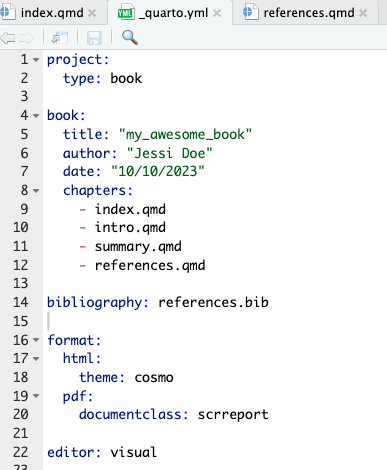
\includegraphics[width=2.08333in,height=\textheight]{img/quarto_intro/Screenshot 2023-10-12 at 11.41.30.png}

\_\_\_\_\_\_\_\_\_\_\_\_\_\_\_\_\_\_\_\_\_\_\_\_\_\_\_\_\_\_\_\_\_\_\_\_\_\_\_\_\_\_\_\_\_\_\_\_\_\_\_\_\_\_\_\_\_\_\_\_\_\_\_\_\_\_\_\_\_\_\_\_\_

With this, you should at least have some ideas on how you can use quarto
in your daily work routine. Happy coding and please feel free to contact
me for any remarks or questions. I am happy to try and help.

\hypertarget{vscode}{%
\section{VSCode}\label{vscode}}

Much of the concepts as described in the RStudio tutorial above apply
equally well to using Quarto in VSCode, just with a different interface
to execute them.

Here we will describe how to set up VSCode and Quarto, and how to
preview and render Quarto objects within the VSCode interface.

To understand about more about the details of which files to edit etc.,
please see the RStudio description above.

\hypertarget{getting-started-1}{%
\subsection{Getting Started}\label{getting-started-1}}

\begin{enumerate}
\def\labelenumi{\arabic{enumi}.}
\tightlist
\item
  Install the Quarto CLI tool for your operating system from the
  \href{https://quarto.org/docs/get-started/}{Quarto Website}
\item
  Install the
  \href{https://marketplace.visualstudio.com/items?itemName=quarto.quarto}{VSCode
  Quarto extension}
\end{enumerate}

\hypertarget{using-quarto}{%
\subsection{Using Quarto}\label{using-quarto}}

The basic workflow is as follows:

\begin{enumerate}
\def\labelenumi{\arabic{enumi}.}
\tightlist
\item
  Create or modify \texttt{.qmd} objects etc as described above in the
  Rstudio section about \protect\hyperlink{qmd-files}{Quarto markdown
  files}
\item
  Within VSCode, make sure you've opened it in the repository containing
  all the files
\item
  Press ctrl + shift + p to bring up your command palette

  \begin{enumerate}
  \def\labelenumii{\arabic{enumii}.}
  \tightlist
  \item
    To preview a local `live' version of HTML or website versions, you
    can type \texttt{Quarto:\ preview}. To close the live preview, press
    ctrl+c in the VSCode terminal.
  \item
    To render all the files e.g.~final HTML and/or PDF versions, you can
    type \texttt{Quarto:\ Render\ Project}, where you will be given
    different options depending on the formats defined in the
    \texttt{\_quarto.yml} file.
  \end{enumerate}
\end{enumerate}

For further VSCode integrations, just type \texttt{Quarto:} into your
command palette and explore all the options.

\bookmarksetup{startatroot}

\hypertarget{references-1}{%
\chapter*{References}\label{references-1}}
\addcontentsline{toc}{chapter}{References}

\markboth{References}{References}

\hypertarget{refs}{}
\begin{CSLReferences}{0}{0}
\end{CSLReferences}



\end{document}
